%%%%%%%%%%%%%%%%%%%%%%%%%%%%%%%%%%%%%%%%%%%%%%%%%%%%%%%%%%%%%%%%%%%%%%
% LaTeX Example: Project Report
%
% Source: http://www.howtotex.com
%
% Feel free to distribute this example, but please keep the referral
% to howtotex.com
% Date: March 2011 
% 
%%%%%%%%%%%%%%%%%%%%%%%%%%%%%%%%%%%%%%%%%%%%%%%%%%%%%%%%%%%%%%%%%%%%%%
% How to use writeLaTeX: 
%
% You edit the source code here on the left, and the preview on the
% right shows you the result within a few seconds.
%
% Bookmark this page and share the URL with your co-authors. They can
% edit at the same time!
%
% You can upload figures, bibliographies, custom classes and
% styles using the files menu.
%
% If you're new to LaTeX, the wikibook is a great place to start:
% http://en.wikibooks.org/wiki/LaTeX
%
%%%%%%%%%%%%%%%%%%%%%%%%%%%%%%%%%%%%%%%%%%%%%%%%%%%%%%%%%%%%%%%%%%%%%%
% Edit the title below to update the display in My Documents
%\title{Project Report}
%
%%% Preamble
\documentclass[paper=a4, fontsize=11pt]{scrartcl}
\usepackage[T1]{fontenc}
\usepackage{fourier}

\usepackage[english]{babel}															% English language/hyphenation
\usepackage[protrusion=true,expansion=true]{microtype}	
\usepackage{amsmath,amsfonts,amsthm} % Math packages
\usepackage[pdftex]{graphicx}	
\usepackage{url}

\usepackage{hyperref}
\usepackage{amsmath}
\usepackage{amsfonts}
\usepackage{amssymb}
\usepackage{graphicx}
\usepackage{nameref}
\usepackage{multicol}
\usepackage{float}
\usepackage{multirow}
\usepackage[ruled, linesnumbered]{algorithm2e}


% \numberwithin{equation}{subsection}
% \renewcommand{\thesubsection}{\thesection.\arabic{subsection}}
% \renewcommand{\thesubsubsection}{\Alph{subsubsection}}
% \newcommand{\setsubsubsectionnumber}[1]{\setcounter{subsubsection}{#1}\addtocounter{subsubsection}{-1}}

\newcommand{\abs}[1]{\vert #1\vert}
\newcommand{\tab}[1][30pt]{\hspace*{#1}}
\newcommand{\bracket}[1]{\biggl[#1\biggr]}
\newcommand{\norm}[1]{\left\lVert #1\right\rVert}


\DeclareMathOperator*{\argmin}{arg\,min}
\DeclareMathOperator*{\argmax}{arg\,max}
\DeclareMathOperator*{\divergance}{D}
\DeclareMathOperator*{\LDS}{LDS}
\DeclareMathOperator*{\sign}{sign}


\newcommand*{\D}[2]{\divergance \left[#1, #2\right]}




%%% Custom sectioning
\usepackage{sectsty}
\allsectionsfont{\centering \normalfont\scshape}


%%% Custom headers/footers (fancyhdr package)
\usepackage{fancyhdr}
\pagestyle{fancyplain}
\fancyhead{}											% No page header
\fancyfoot[L]{}											% Empty 
\fancyfoot[C]{}											% Empty
\fancyfoot[R]{\thepage}									% Pagenumbering
\renewcommand{\headrulewidth}{0pt}			% Remove header underlines
\renewcommand{\footrulewidth}{0pt}				% Remove footer underlines
\setlength{\headheight}{13.6pt}


%%% Equation and float numbering
\numberwithin{equation}{section}		% Equationnumbering: section.eq#
\numberwithin{figure}{section}			% Figurenumbering: section.fig#
\numberwithin{table}{section}				% Tablenumbering: section.tab#


%%% Maketitle metadata
\newcommand{\horrule}[1]{\rule{\linewidth}{#1}} 	% Horizontal rule

\title{
		%\vspace{-1in} 	
		\usefont{OT1}{bch}{b}{n}
		\normalfont \normalsize \textsc{Electrical Engineering Department, Sharif University of Technology} \\ [25pt]
		\horrule{0.5pt} \\[0.4cm]
		\huge VAT: Virtual Adversarial Training \\
		\horrule{2pt} \\[0.5cm]
}
\author{
		\normalfont 								\normalsize
        Ali Abbasi\\[-3pt]		\normalsize
        February 11, 2023
}
\date{}


%%% Begin document
\begin{document}
\maketitle
\section{Abstract}
In this report, we present a new regularization technique called Virtual Adversarial Training (VAT). VAT is based on the virtual adversarial loss, which evaluates the local smoothness of the conditional label distribution with respect to the input data. Unlike traditional adversarial training, our method determines the adversarial direction without using label information, making it appropriate for semi-supervised learning. The virtual adversarial direction is used to smooth the model in this technique. The computation cost of VAT is low, as the gradient of the virtual adversarial loss can be calculated using just two forward and backward propagation for neural networks. Our experiments demonstrate that VAT can be    applied to both supervised and semi-supervised learning tasks on multiple benchmark datasets. With a slight modification based on the entropy minimization principle, VAT surpasses current state-of-the-art methods for semi-supervised learning on the SVHN and CIFAR-10 datasets.


\section{Introduction}
In this Section, some of the main definitions are explained.
\subsection{Adversarial Attacks}
These attacks cause a machine-learning model to make incorrect predictions. this is achieved by adding perturbations to inputs that degrade the information in an input signal. Deep learning systems are vulnerable to adversarial attacks. Their outputs can be manipulated with imperceptibly small perturbations applied to the inputs.
\subsection{Optimal Adversarial Attack}
Optimal adversarial attack maximally degrades the achievable performance of the system as measured by the mutual information between the degraded signal and the label of interest.\\
\\
Consider random variable $U$ to denote the quantity (or label) of interest. The random variable $X \in R$ denotes the data generated from $U$. 
We aim to minimize the mutual information between $U$ and $Y$, where $Y$ is a random variable that results from adding a random perturbation $E$ to $X$. To minimize the costs associated with adding perturbations, we impose constraints on $E$. For instance, to ensure that the perturbation is not noticeable, we can set a constraint that its expected $l_2$ norm is less than a specified threshold, such as $\epsilon$. The overall design of the proposed model is shown in Figure 2.1.
\\
\\
Suppose $(U, X)$ and $(U, X, E)$ be jointly distributed according to distributions $p(U, X)$ and $p(U, X, E)$, respectively. therefore, the problem is as follows:
\begin{align}
\min_{p(E|U,X)\in \mathcal{P}} I(U;X+E) \equiv \max_{p(E|U,X)\in \mathcal{P}} H(U|X+E)
\end{align}
\begin{center}
    $[Note: \qquad I(U;X+E) = H(U) - H(U|X+E)]$
\end{center}

\\
where $\mathcal{P}$ is a set of admissible probability distributions.
\newline
for example, it can be:
\begin{align}
\mathcal{P} &= \{p(E|U,X): \mathbb{E}[\norm{E}^2] \leq \epsilon, X \in \Omega\}
\end{align}


\begin{figure}
\centering
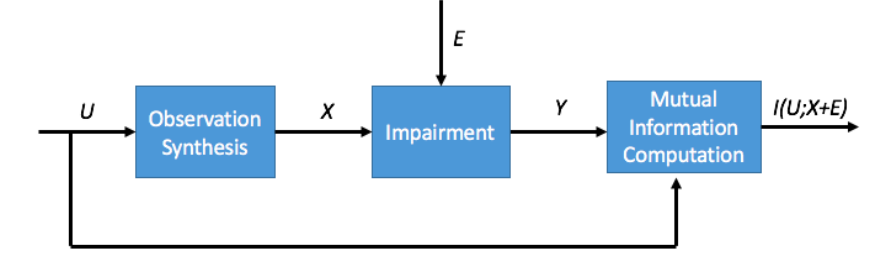
\includegraphics[width=0.8\columnwidth]{first paper.png}
\caption{Mutual information-based framework for adversarial attacks}
\end{figure}

\subsubsection{The Case of Gaussian Random Variables}
In this section, the optimal adversarial attack problem is solved in scenarios where U follows a Gaussian distribution.
\\

$Theorem 2.2.1$. Suppose that random variable $U \in R$ follows Gaussian distribution $N(0, a^2)$. Let random
variable $W$ follow Gaussian distribution $N(0, \sigma^2
)$, and be independent of $U$. The data $X = U + W$. Let $D$
be a non-negative number. Under the constraint that the perturbation $E$ satisfies $E{E2} \leq D$, the optimal
perturbation E that minimizes the mutual information $I(U; U+W+E)$, is jointly Gaussian distributed with
$U$ and $W$, and has zero mean. Moreover, under the optimal distribution, the covariance matrix of $(U, W, E)$
is given by:[cite to our first reference paper]

\begin{align}
    F = 
    \begin{bmatrix}
    a^2 & 0 & x\\
    0 & \sigma^2 & y\\
    x & y & D
    \end{bmatrix}
\end{align}

where $(x, y)$ is the optimal solution to the following optimization problem:
\begin{align}
  min_{x, y} \frac{(a^2+x)^2}{a^2(a^2+\sigma^2+D+2y+2x)}    \end{align}

\begin{center}
  $s.t$ \quad $\frac{x^2}{a^2} + \frac{y^2}{\sigma^2} \leq D$  
\end{center}
$proof$: Let us assume that $F$ is the covariance matrix of $(U, W, E)$, then the covariance
matrix of $(U + W + E, U)$ is given by:

\begin{align}
    G = 
    \begin{bmatrix}
    a^2+\sigma^2+D+2y+2x  & a^2+x\\
    a^2+x & a^2
    \end{bmatrix}
\end{align}

if $Z = U -\frac{G_{21}}{G_{11}}(U+W+E)$, then $var(Z) = G_{22} - \frac{G_{21}}{G_{11}} (G_{12})$. Then we have the below inequality:

\begin{align}
    I(U+W+E;U) &= h(U) - h(U|U+W+E) \\
    &= h(U) - h(Z|U+W+E) \\
    &\geq h(U) - h(Z) \\
    &\geq h(U) - h(Z_g) \\
     &=\frac{1}{2} log(2\pi e a^2) - \frac{1}{2} log(2\pi e(G_{22} - G_{21}G_{11}^{-1}G_{12})) \\
     &=\frac{1}{2} log(2\pi e a^2) - \frac{1}{2} log(2\pi e (a^2 - \frac{(a^2+x)^2}{a^2+\sigma^2+D+2y+2x}))\\
     &= - \frac{1}{2} log(1 - \frac{(a^2+x)^2}{a^2(a^2+\sigma^2+D+2y+2x)}) 
\end{align}

Let $Z_g$ be a Gaussian random variable with the same mean and variance as $Z$. The maximum value of $h(Z)$ is obtained when $Z$ follows a Gaussian distribution. Furthermore, when $(U, V, W)$ are zero-mean Gaussian random variables with covariance matrix $F$, the mutual information between $I(U; U + W + E)$ can achieve $- \frac{1}{2} log(1 - \frac{(a^2+x)^2}{a^2(a^2+\sigma^2+D+2y+2x)}) $. The smallest achievable value
of $I(U; U + W + E)$ is thus given by the following optimization problem:\\
\begin{align}
   min_{x, y} - \frac{1}{2} log(1 - \frac{(a^2+x)^2}{a^2(a^2+\sigma^2+D+2y+2x)}) 
\end{align}

\begin{center}
  $s.t \quad 
  \begin{bmatrix}
    a^2 & 0 & x\\
    0 & \sigma^2 & y\\
    x & y & D
    \end{bmatrix}
     \succeq 0$  
\end{center}

By the Schur complement, the condition that $F\succeq 0$ is equivalent to $\frac{x^2}{a^2} + \frac{y^2}{\sigma^2} \leq D$, From the monotonicity of $- \frac{1}{2} log(1-x)$ in x, the solution minimizing the objective function in the above optimization problem will also be the minimizer of our objective function.




\subsection{Robustness}
The ability of a model to produce accurate and trustworthy results even in the presence of unexpected or abnormal inputs.
\\
\\
Robustness is important because of several reasons. Firstly, confidence in any tool is contingent upon its consistent and dependable operation. This trust can be undermined when an ML system behaves in an unexpected manner that is challenging to comprehend. Secondly, deviations from expected performance can signal crucial issues that demand attention, such as malicious attacks, unforeseen events, undiscovered biases, or substantial changes in the data. To guarantee that a model is fulfilling its intended function, it is essential to examine, keep track of, and maintain its robustness as part of model risk management.

\subsection{Semi-Supervised Learning}
Currently, there exist vast datasets composed mainly of unlabeled data. Labeling these datasets is both time-consuming and costly, making it increasingly crucial to develop methods for semi-supervised learning and the unlabeled data can be used to help the training.
\\
\\
Semi-supervised learning is a machine learning technique that combines both supervised and unsupervised learning. In supervised learning, the model is trained with labeled data. On the other hand, in unsupervised learning, the model is only provided with inputs and must find patterns or relationships in the data without any labeled output.
\\
\\
Semi-supervised learning combines these two approaches by using a small amount of labeled data and a large amount of unlabeled data. The model is trained on the labeled data and uses this knowledge to make predictions on the unlabeled data. This can help improve the model's accuracy and generalization performance, as well as reduce the amount of labeled data needed to train the model.

\subsection{Regularization}
Regularization helps to control the complexity of a model by adding a penalty term to the loss function that is being optimized. This term discourages the model from assigning large weights to any of its features, reducing the risk of over-fitting. As a result, regularized models are more robust to variations in the input data, making them better equipped to handle unseen data. By adding the penalty term, regularization ensures that the model focuses on capturing the underlying structure of the data, rather than fitting to the noise in the training set, which leads to improved generalization.
\\
\\
From a Bayesian standpoint regularization can be interpreted as a prior distribution that reflects our educated a priori knowledge or belief regarding the model. 
\\
\\
It is a widely accepted belief, based on observed facts, that the outputs of most naturally occurring systems exhibit smoothness with respect to their spatial and/or temporal inputs.

\section{Related Works}
In this section, we summarize the most relevant papers.
\subsection{"Learning from labeled and unlabeled data with label propagation" \cite{Learning from labeled and unlabeled data with label propagation}}
The paper "Learning from Labeled and Unlabeled Data with Label Propagation" presents a semi-supervised learning method for classifying data using both labeled and unlabeled samples. The method, called Label Propagation, works by propagating class labels from labeled samples to unlabeled samples through a graph-based representation of the data. The method takes into account the similarity between samples, as well as the agreement between the predicted labels and the true labels of the labeled samples.
\\
\\
In essence, Label Propagation uses the labeled samples to guide the classification of the unlabeled samples. This allows the model to make use of additional information beyond just the labeled samples, leading to improved performance in comparison to purely supervised learning methods that only use labeled samples.
\\
\\
The authors evaluate the performance of Label Propagation on several benchmark datasets and show that it outperforms other semi-supervised learning methods, as well as standard supervised learning methods that use only labeled data.
\\
\\
Overall, the paper highlights the effectiveness of using both labeled and unlabeled data in semi-supervised learning and provides a useful framework for researchers and practitioners looking to solve classification problems with limited labeled data.

\subsection{"Explaining and Harnessing Adversarial Examples" \cite{Explaining and harnessing adversarial examples}}
The paper "Explaining and Harnessing Adversarial Examples" is a seminal work in the field of adversarial machine learning. It discusses the phenomenon of adversarial examples, where small, seemingly insignificant perturbations to inputs can cause a machine learning model to produce incorrect outputs.
\\
\\
The authors show that these adversarial examples are not simply random noise, but rather systematic manipulations of the input data that are specifically crafted to fool the model. They present a method for generating these adversarial examples, called the Fast Gradient Sign Method (FGSM), which computes the gradient of the loss function with respect to the input and uses it to generate adversarial examples.
\\
\\
The paper also provides an explanation for why adversarial examples exist, stating that the robustness of machine learning models is limited by their linear nature. In other words, models are vulnerable to adversarial examples because they are only capable of making linear predictions, and cannot capture the non-linear relationships in the data.
\\
\\
The authors then present a defense method called adversarial training, which involves adding adversarial examples to the training data to improve the robustness of the model. They show that this method can improve the performance of the model on adversarial examples and increase its overall robustness.
\\
\\
Overall, the paper provides a thorough understanding of adversarial examples and their implications for machine learning models. It serves as a starting point for researchers and practitioners looking to improve the robustness and security of machine learning models against adversarial attacks.

\subsection{"Intriguing Properties of Neural Networks" \cite{ Intriguing properties of neural networks}}
The paper "Intriguing Properties of Neural Networks" explores some of the intriguing properties of deep neural networks and how they can be used for both positive and negative purposes.
\\
\\
One of the key findings of the paper is that neural networks can be highly susceptible to adversarial examples, small but carefully crafted input perturbations that cause the network to make incorrect predictions. The authors demonstrate that these adversarial examples can be generated with relative ease, and can be used to mislead deep learning models in various applications, such as image classification, speech recognition, and autonomous driving.
\\
\\
The paper also shows that deep neural networks have the ability to memorize training data, even when the training data is randomly generated or noisy. This means that deep learning models can achieve high accuracy on the training set, but have poor generalization performance on new, unseen data.
\\
\\
Overall, "Intriguing Properties of Neural Networks" highlights the potential and limitations of deep learning models, and provides insights into the development of more robust and secure deep learning architectures. The findings of this paper have since sparked numerous research studies on the robustness and security of deep learning models and their applications.

\subsection{"Learning with Pseudo-Ensembles" \cite{Learning with pseudo-ensembles}}
The paper "Learning with Pseudo-Ensembles" presents a semi-supervised learning method that combines the strengths of both supervised and unsupervised learning. The method, called pseudo-ensembles, works by training multiple models on different subsets of labeled data and combining their predictions for unlabeled data to produce a more accurate final prediction.
\\
\\
The key idea behind pseudo-ensembles is that by training multiple models on different subsets of the data, each model can learn different patterns and representations of the data. When combined, these models can provide a more diverse set of predictions, which can lead to improved performance on the final prediction task.
\\
\\
The authors show that pseudo-ensembles outperform both supervised and unsupervised learning methods on several benchmark datasets. Additionally, they demonstrate that the method can be applied to both traditional machine learning algorithms, such as decision trees and neural networks, and modern deep learning models.
\\
\\
Overall, the paper provides a valuable contribution to the field of semi-supervised learning and highlights the importance of combining labeled and unlabeled data for improved performance. It is a useful reference for researchers and practitioners looking to improve the accuracy of their predictions on large, real-world datasets with limited labeled data.

\subsection{"Unsupervised and Semi-Supervised Learning with Categorical Generative Adversarial Networks" \cite{Unsupervised and semi-supervised learning with categorical generative adversarial networks}}
"Unsupervised and Semi-Supervised Learning with Categorical Generative Adversarial Networks" explores the use of generative adversarial networks (GANs) for unsupervised and semi-supervised learning tasks. In this paper, the authors propose a novel variant of GANs, known as Categorical Generative Adversarial Networks (CatGANs), which are designed to handle categorical data, such as image labels or text categories.
\\
\\
CatGANs consist of a generator network and a discriminator network, which are trained together in an adversarial manner. The generator network generates samples from a learned latent space, while the discriminator network tries to distinguish between real and fake samples. The authors show that CatGANs can be trained in an unsupervised manner, where the generator learns to generate samples that are similar to the training data, and in a semi-supervised manner, where the generator learns to generate samples that belong to a specific category.
\\
\\
The authors also evaluate the performance of CatGANs on several benchmark datasets and compare the results with other unsupervised and semi-supervised learning methods. They show that CatGANs can achieve good results in both unsupervised and semi-supervised learning scenarios, and outperform other methods in some cases.
\\
\\
In conclusion, "Unsupervised and Semi-Supervised Learning with Categorical Generative Adversarial Networks" is a significant contribution to the field of deep learning, as it demonstrates the potential of CatGANs for unsupervised and semi-supervised learning tasks and highlights the importance of considering the structure of the data when designing deep learning models.

\subsection{"TOWARDS DEEP NEURAL NETWORK ARCHITECTURES ROBUST TO ADVERSARIAL EXAMPLES"\cite{Towards deep neural network architectures robust to adversarial example}}
The paper "Towards Deep Neural Network Architectures Robust to Adversarial Examples" focuses on improving the robustness of deep neural networks (DNNs) against adversarial examples. The authors study the structure of adversarial examples and explore various techniques such as network topology, pre-processing, and training strategies to improve the robustness of DNNs. The authors also perform experiments to assess the removal of adversarial examples using denoising autoencoders (DAEs). However, they find that stacking the DAE with the original DNN can lead to new adversarial examples with even smaller distortion. To address this issue, the authors propose a new end-to-end training procedure called "Deep Contractive Network" which includes a smoothness penalty inspired by the contractive autoencoder (CAE) that increases the network's robustness against adversarial examples.

\section{Method}
In this section, we establish some notation. Let $x \in R^I$ and $y$ be an output label in $Q$, where $I$ represents the input dimension and $Q$ represents the set of all possible labels. The output distribution, parameterized by $\theta$, is denoted as $p(y|x, \theta)$. The parameter vector of the model at a particular training iteration is represented by $\hat{\theta}$. A labeled dataset is represented as $D_l = {(x_l^{(n)}, y_l^{(n)})|n = 1, ..., N_l}$, and an unlabeled dataset is represented as $D_{ul} = {x_l^{(n)} |m = 1, ..., N_{ul}}$. We will use both the labeled dataset $D_l$ and the unlabeled dataset  $D_{ul}$ to train the model $p(y|x, \theta)$.

\subsection{Adversarial Training \cite{Intriguing
properties of neural networks}}
Our approach closely aligns with the adversarial training concept. To provide context, we will first describe the adversarial training before presenting our method. The loss function for adversarial training can be expressed as follows:
\begin{align}
\label{eq:loss}L_{adv}(x_l, \theta) &= \D{q(y | x_l)}{p(y | x_l + r_{adv}, \theta)}
\end{align}
\begin{align}
\label{eq:appradv} \text{where } \quad r_{adv} &= \argmax_{r; \norm{r} \le \epsilon} \D{q(y | x_l)}{p(y | x_l + r, \theta)} 
\end{align}
Where $D[p, p']$ is a non-negative function that calculates the difference between two distributions $p$ and $p'$. For instance, $D$ can be the cross entropy. The function $q(y|x_l)$ represents the true distribution of the output label, which is unknown. The aim of the loss function is to approximate the true distribution $q(y|x_l)$ using a parametric model $p(y|x, \theta)$ robust against adversarial attack to $x$. In this section, the true distribution $q(y|x_l)$ is estimated using a one-hot vector $h(y;y_l)$, in which all entries are zero except for the index corresponding to the true label $y_l$. 
\\
\\
It is not possible to obtain a closed form for the exact adversarial perturbation $r_adv$. However, a linear approximation of $D$ with respect to $r$ in the Eq.\eqref{eq:appradv} can be used to approximate $r_adv$. When the norm is $L_2$, the adversarial perturbation can be estimated by:
\\
\begin{align}
\label{eq:radv}r_{adv} &\approx \epsilon \frac{g}{\norm{g}_2}
\end{align}
\begin{center}
$where \quad g = \nabla_{x_l} \D{h(y ; y_l)}{p(y | x_l, \theta)}$\\
\end{center}
$proof:$ The first-degree Taylor series approximation of $r_{adv}^*$, the solution to the optimization problem given in Eq.\eqref{eq:appradv}, is written as follows:
\begin{align}
r_{adv}^* = r_{adv} + \langle r_{adv},\nabla_{x_l} \D{h(y ; y_l)}{p(y | x_l, \theta)}\rangle
\end{align}
To maximize this expression $r_{adv}$ needs to be in $\nabla_{x_l} \D{h(y ; y_l)}{p(y | x_l, \theta)}$ direction.
\\
\\
It is important to note that $\nabla_{x_l} \D{h(y ; y_l)}{p(y | x_l, \theta)}$ for neural networks can be efficiently computed using backpropagation. By optimizing the loss function of adversarial training Eq.\eqref{eq:loss} with the adversarial perturbation defined in Eq.\eqref{eq:radv}, researchers have shown that models can be trained with improved generalization performance compared to models trained with random perturbations.


\subsection{Virtual Adversarial Training}
As we saw, adversarial training is a method for training robust models which is successful in many cases.
However, it depends on the full label information of the data. 
Thus, it cannot be used in semi-supervised settings.
In this part, we describe the Vritual Adversarial Training (VAT) method, which solves this problem.
Let \(x_*\) represent either a labeled (\(x_l\)) or unlabeled (\(x_{ul}\)) data point.
Our objective function is:
\begin{align}
&\D{q(y | x_*)}{p(y | x_* + r_{qadv}, \theta)}\\
\text{Where: } &r_{qadv} = \argmax_{r; \norm{r} \le \epsilon} \D{q(y | x_*)}{p(y | x_* + r, \theta)}
\end{align}
But there is no direct information about \(q(y | x_{ul})\) and this time, one-hot vector of the label cannot be used as an approximation for it.
So instead, its current approximation is used, i.e. \(p(y | x_*, \hat{\theta})\).
This is why the term ``virtual'' is used in the name of the method.
With this approximation, we arrive at the Eq.~\eqref{eq:vat1} as follows:
\begin{align}
\label{eq:vat1}
\LDS(x_*, \theta) &= \D{p(y | x_*, \hat{\theta})}{p(y | x_* + r_{vadv}, \theta)}\\
r_{vadv} &= \argmax_{r; \norm{r} \le \epsilon} \D{p(y | x_*, \hat{\theta})}{p(y | x_* + r, \theta)}
\end{align}
Where \(\LDS\) is the \textit{Local Distributional Smoothness}, which can be considered as a negative measure of local smoothness of model at each data point.
The regularization term is simply the average of \(\LDS\) over all data points:
\begin{align}
\mathcal{R}(\mathcal{D}_l, \mathcal{D}_{ul}, \theta) = \frac{1}{N_l + N_{ul}} \sum_{x_* \in \mathcal{D}_l, \mathcal{D}_{ul}} \LDS(x_*, \theta)
\end{align}
And the full objective becomes:
\begin{align}
\mathcal{L} = \ell(D_l, \theta) + \alpha \mathcal{R}(D_l, D_{ul}, \theta)
\end{align}
Where \(\ell(D_l, \theta)\) is the negative log-likelihood of the labeled data and \(\alpha\) is a hyperparameter that controls the strength of the regularization term.

\subsection{Approximating \(r_{vadv}\) and the Derivative of the Objective function}
As one can see, the \(LDS(x_*, \theta)\) is now is divergence \(D\) between the distributions \(p(y | x_*, \hat{\theta})\) and \(p(y | x_* + r, \theta)\).
But unlike the adversarial training, this divergence cannot be approximated using simple first degree Taylor expansion. Because the value of divergence is now always zero at \(r = 0\).\\
Let us denote \(\D{p(y | x_*, \hat{\theta})}{p(y | x_* + r, \theta)}\) with \(\divergance(r, x_*, \hat{\theta})\).
We know that \(\divergance(r, x_*, \hat{\theta})\) takes its minimum value ate \(r=0\). 
With assuming \(p(y|x_*, \theta)\) to be twice differentiable with respect to \(x_*\) and \(\theta\) in almost everywhere, we can infer conclude that \(\nabla_r \divergance(r, x, \hat{\theta})|_{r=0} = 0\).
Considering this, we can write the second-order Taylor expansion of \(\divergance\) as:
\begin{align}
  \divergance(r, x, \hat{\theta}) \approx \frac{1}{2} r^T H(x, \hat{\theta})r
\end{align}
Where \(H(x, \hat{\theta})\) is the Hessian matrix of \(\divergance\) with respect to \(r\).
Using this second-order approximation, we can see that \(r_{vadv}\) emerges to be the dominant eigenvector of the Hessian matrix \(H(x, \hat{\theta})\):
\begin{align}
  r_{vadv} &\approx \argmax_r\left\{r^T H(x, \hat{\theta})r \mid \norm{r} \le \epsilon\right\}\\
  &= \epsilon \overline{u(x, \hat{\theta})}
\end{align}
Where \(u(x, \hat{\theta})\) is the dominant eigenvector of \(H(x, \hat{\theta})\) and \(\overline{u}\) is its unit vector.

In order to avoid \(O(I^3)\) cost of computing the dominant eigenvector of \(H\), the authors propose to use the power iteration method, which is the multiple application the following matrix-vector multiplication:
\begin{align}
\label{eq:power_iteration}
d \gets \overline{Hd}
\end{align}
Where in the first iteration, \(d\) is initialized to a random unit vector.
Assuming that the first random vector is not orthogonal to the dominant eigenvector, it can be shown that the power iteration method converges to the dominant eigenvector of \(H\):
Suppose \(v_1, v_2, \ldots, v_n\) are eigenvectors of \(H\) sorted by their eigenvalues in descending order.
Then, the power iteration method converges to \(v_1\) as follows:
\begin{align}
\text{Suppose } d_0 &= c_1 v_1 + c_2 v_2 + \cdots + c_n v_n\\
\implies d_k &= Hd_{k-1} = H^k d_0 = H^k (c_1 v_1 + A^k c_2 v_2 + \cdots + A^k c_n v_n)\\
&= \lambda_1^k c_1 v_1 + \lambda_2^k c_2 v_2 + \cdots + \lambda_n^k c_n v_n\\
&= \lambda_1^k (c_1 v_1 + \left(\frac{\lambda_2}{\lambda_1}\right)^k c_2 v_2 + \cdots + \left(\frac{\lambda_n}{\lambda_1}\right)^k c_n v_n)\\
&\xrightarrow[]{k \to \infty} \lambda_1^k c_1 v_1
\end{align}
So the repetition of Eq.~\eqref{eq:power_iteration} converges to the \(\overline{u}\).

Now we use another approximation for computing \(Hd\) too with the difference method:
\begin{align}
  Hd &\approx \frac{\nabla_r \divergance(r, x_*, \hat{\theta})|_{r=\xi d} - \nabla_r \divergance(r, x_*, \hat{\theta})|_{r=0}}{\xi}\\
  &= \frac{\nabla_r \divergance(r, x_*, \hat{\theta})|_{r=\xi d}}{\xi}
\end{align}
Where \(\xi\) is a small constant. And in the second line, we used the fact that \(\nabla_r \divergance(r, x_*, \hat{\theta})|_{r=0} = 0\) again. Thus, the iteration becomes:
\begin{align}
\implies d \leftarrow \overline{\nabla_r \divergance(r, x_*, \hat{\theta})|_{r=\xi d}}
\end{align}
And in each iteration, the gradient of \(\divergance\) is computed using backpropagation in the neural network.
The authors showed that only one iteration of the power method resulted to a good enough model for various datasets (see table \ref{tab:different_K}).
Algorithm \ref{alg:vat_k1} shows the pseudo code of the proposed method for one iteration of power method.

\begin{algorithm}
\label{alg:vat_k1}
\caption{Mini-batch SGD for \(\nabla_\theta\mathcal{R}\) with one time iteration of power method}
Choose \(M\) random samples from dataset \(\mathcal{D}\): \(\left\{x^{(i)}\right\}_{i=1}^M\).\\
Sample unit vector \(d^{(i)}\) from an iid Gaussian distribution.\\
Calculate \(r_{vadv}\) with one set of backpropagation:
\begin{align*}
g^{(i)} &\gets \left.\nabla_r \D{p(y | x^{(i)}, \hat{\theta})}{p(y | x^{(i)} + r, \theta)}\right|_{r=\xi d^{(i)}}\\
r_{vadv}^{(i)} &\gets \epsilon \frac{g^{(i)}}{\norm{g^{(i)}}}
\end{align*}\\
\Return{\(\nabla_\theta \left(\frac{1}{M}\sum_{i=1}^M \D{p(y | x^{(i)}, \hat{\theta})}{p(y | x^{(i)} + r_{adv}^{(i)}, \theta)}\right)\)}
\end{algorithm}

It is worth mentioning how the hyperparameter tuning is done for vat before we move on to the experiments.
As mentioned, there are two hyperparameters in the proposed method: \(\epsilon\) and \(\alpha\).
But we can show that tuning only one of them is enough.

As we saw:
\begin{align}
\max_r\left\{ \divergance(r, x, \theta) \mid \norm{r}_2 \le \epsilon\right\} & \approx \max_r\left\{\frac{1}{2} r^T H(x, \theta)r \mid \norm{r}_2 \le \epsilon\right\}\\
& = \frac{1}{2} \epsilon^2 \lambda_1(x, \theta)
\end{align}
Where \(\lambda_1(x, \theta)\) is the dominant eigenvalue of \(H(x, \theta)\).
Substituting this into the objective function, we get:

\begin{align}
\mathcal{L} &= \ell(\theta, \mathcal{D}_l) + \alpha \mathcal{R}_{vadv} (\theta, \mathcal{D}_l, \mathcal{D}_{ul})\\
&= \ell(\theta, \mathcal{D}_l) + \alpha \frac{1}{N_l + N_{ul}} \sum_{x \in \mathcal{D}_l, \mathcal{D}_{ul}} \max_r\left\{ \divergance(r, x, \theta) \mid \norm{r}_2 \le \epsilon\right\}\\
& \approx \ell(\theta, \mathcal{D}_l) + \frac{1}{2} \epsilon^2\alpha \frac{1}{N_l + N_{ul}} \sum_{x \in \mathcal{D}_l, \mathcal{D}_{ul}}  \lambda_1(x, \theta)
\end{align}
And we can see that the strength of the regularization term is proportional to \(\epsilon^2\alpha\).
Which means we can fix the value of one of \(\alpha\) or \(\epsilon\) and tune the other one.
In the experiments that we are going to explain, \(\alpha\) is fixed to 1 and \(\epsilon\) is tuned.

\section{Experiment}
A set of experiments are done to show the effectiveness of the proposed method.
In these experiments, KL divergence is used as the divergence \(\divergance\) and \(\xi\) in Eq.~\eqref{eq:power_iteration} is set to $10^{-6}$.
Moreover, for each experiment the same procedure was repeated multiple times with different random seeds for the weight initialization and the random samples of labeled data and the means and standard deviations of the test accuracies are reported.

For the MNIST dataset, Virtual Adversarial Training method was applied to a simple neural network with four hidden layers of size 1200, 600, 300, 150.
For each experiment, the hyperparameters were chosen that achieved the best performance on the validation set. Table \ref*{tab:mnist} summarizes the result of this part.

\begin{table}[H]
\centering
\caption{Test performance of supervised learning methods
on MNIST with 60,000 labeled examples in the permutation
invariant setting.}
\label{tab:mnist}
\begin{tabular}{l r}
\hline
\hline
Method & Test error rate(\%)\\
\hline
SVM (Gaussian kernel) & 1.40\\
Dropout  & 1.05\\
Adversarial, \(L_\infty\) norm constraint &  0.78\\
Ladder networks &  0.57 (\(\pm\)0.02)\\
\hline
Baseline (MLE) & 1.11 (\(\pm\)0.06)\\
RPT & 0.84 (\(\pm\)0.03)\\
Adversarial, \(L_1\) norm constraint &0.79 (\(\pm\)0.03)\\
Adversarial, \(L_2\) norm constraint& 0.71 (\(\pm\)0.03)\\
VAT &0.64 (\(\pm\)0.05)\\
\hline
\hline
\end{tabular}
\end{table}

As you can see, VAT outperforms all the other methods in this setting, except for the Ladder network. This was expected since Ladder networks is a highly advanced method based on special network structure, and VAT could achieve comparable results with this network with a very simple architecture.

The authors also tested their method with supervised learning setting on CIFAR10 dataset too. For this part, Conv-Large %TODO
with dropout was used as the baseline network (see Table~\ref{tab:ciphar10}).

\begin{table}[H]
\label{tab:ciphar10}
\centering
\caption{Test performance of supervised learning methods
implemented with CNN on CIFAR-10 with 50,000 labeled
examples.}
\label{tab:ciphar10}
\begin{tabular}{l r}
\hline
\hline
Method & Test error rate(\%)\\
\hline
Network in Network & 8.81\\
All-CNN & 7.25\\
Deeply Supervised Net & 7.97\\
Highway Network & 7.72\\
ResNet (1001 layers) & 4.62 (\(\pm\)0.20)\\
DenseNet (190 layers) & 3.46\\
\hline
Baseline (only with dropout) &6.67 (\(\pm\)0.07)\\
RPT &6.30 (\(\pm\)0.04)\\
VAT &5.81 (\(\pm\)0.02)\\
\hline
\hline
\end{tabular}
\end{table}

In this experiment, advanced networks like ResNet and DenseNet were used too, to show that the effectiveness of the VAT is due to its regularization method and not the structure of the network.

And finally, VAT's performance was compared with various models specialized for semi-supervised learning problems with Conv-Small and Conv-Large networks on SVHN and CIFAR10 datasets.
Table \ref{tab:semisup} shows the results of this part.

\begin{table}[H]
\centering
\caption{Test performance of semi-supervised learning
methods.}
\label{tab:semisup}
\resizebox{0.75\columnwidth}{!}{%
\begin{tabular}{l r r}
\hline
\hline
\multirow{3}{*}{Method} & \multicolumn{2}{c}{Test error rate(\%)}\\
& SVHN & CIFAR-10 \\
& \(N_l = 1000\) & \( N_l = 4000\)\\
\hline
SWWAE & 23.56&\\
% *Auxiliary DGM & 22.86&\\
% *Skip DGM & 16.61 (\(\pm\)0.24)&\\
Auxiliary DGM & 22.86&\\
Skip DGM & 16.61 (\(\pm\)0.24)&\\
Ladder networks, \(\Pi\) model && 20.40 (\(\pm\)0.47)\\
CatGAN && 19.58 (\(\pm\)0.58)\\
GQAN with FM & 8.11 (\(\pm\)1.3) &18.63 (\(\pm\)2.32)\\
model & 5.43 (\(\pm\)0.25) &16.55 (\(\pm\)0.29)\\
\hline
(on Conv-Small) & & \\
RPT & 8.41 (\(\pm\)0.24) & 18.56 (\(\pm\)0.29)\\
VAT & 6.83 (\(\pm\)0.24) & 14.87 (\(\pm\)0.13)\\
\hline
(on Conv-Large) & & \\
VAT & 5.77 (\(\pm\)0.32) & 14.18 (\(\pm\)0.38)\\
VAT+EntMin & 4.28 (\(\pm\)0.10)  & 13.15 (\(\pm\)0.21)\\
\hline
\hline
\end{tabular}%
}
\end{table}

As you can see in the table, the VAT+EntMin method outperforms all the other methods, including the advanced and state-of-the-art methods like GAN-based models and Ladder networks.
By EntMin was a method proposed in `Semi-supervised learning by entropy minimization' by Grandvalet et al. (2004).
It adds a simple regularization term to the loss function, \(\mathcal{R}_{cent}\) minimizing the conditional entropy \(\mathcal{H}(Y|X)\) of the output distribution (Eq.~\eqref{eq:entmin}). This makes the model make more confident predictions, and it is shown to improve the performance of semi-supervised learning methods.

\begin{align}
  \label{eq:entmin}
  \mathcal{R}_{cent} &= \mathcal{H}(Y|X)\\
  &= -\frac{1}{N_l + N_{ul}} \sum_{x\in \mathcal{D}_l, \mathcal{D}_{ul}}\sum_{y} p(y|x, \theta) \log p(y|x, \theta)
\end{align}

\subsection{Effect of the Number of the Power Iterations \(K\)}
Table~\ref{tab:different_K} shows the test accuracies of VAT for the semi-supervised learning task on CIFAR10 with different values of \(K\).
As shown in this table, no noticeable improvement could be observed by increasing the number of the power iterations in this dataset.
But there is no guarantee that this will be the case for other datasets too.

\begin{table}[H]
  \label{tab:different_K}
  \centering
  \caption{The test accuracies of VAT for the semi-supervised
  learning task on CIFAR10 with different values of K (the
  number of the power iterations).}
\label{tab:different_K}
\begin{tabular}{l r}
\hline
\hline
& Test error rate(\%)\\
& CIFAR-10\\
& \(N_l = 4000\)\\
\hline
(Using Conv-Large)&\\
VAT, \(K = 1\) & \(14.18 (\pm0.38)\)\\
VAT, \(K = 2\) & \(14.19 (\pm0.16)\)\\
VAT, \(K = 4\) & \(14.25 (\pm0.18)\)\\
\hline
\hline
\end{tabular}
\end{table}

\section{Conclusion}
In this report first we reviewed several famous approaches for training deep neural networks to be robust to adversarial examples.
Then we introduced the VAT method and investigated its effectiveness on various datasets and against various state-of-the-art methods.
We can summarize the advantages of this method as follows:
\begin{itemize}
\item Effective model for both supervised and semi-supervised learning on different datasets
\item Small computational cost
\item Model agnostic
\item Simple:
\begin{itemize}
\item Requires optimization of only one hyperparameter
\item Does not require training of additional models
\end{itemize}
\end{itemize}

\begin{thebibliography}{9}

\bibitem{Virtual Adversarial Training: A Regularization Method for Supervised and Semi-Supervised Learning} Takeru Miyato, Shin-ichi Maeda, Masanori Koyama, Shin Ishii. ``Virtual Adversarial Training: A Regularization Method for Supervised and Semi-Supervised Learning", 2018.
    \bibitem{Derivation of Information-Theoretically Optimal Adversarial Attacks with Applications to Robust Machine Learning} Jirong Yi, Raghu Mudumbai, Weiyu Xu. ``Derivation of Information-Theoretically Optimal Adversarial Attacks with Applications to Robust Machine Learning", 2020.
    \bibitem{Towards deep neural network architectures robust to adversarial example} Shixiang Gu, Luca Rigazio. ``Towards deep neural network architectures robust to adversarial examples", 2015.
    \bibitem{Unsupervised and semi-supervised learning with categorical generative adversarial networks} Jost Tobias Springenberg, ``Unsupervised and semi-supervised learning with categorical generative adversarial networks", 2015.
    \bibitem{Semi-supervised learning by entropy minimization} Yves Grandvalet, Yoshua Bengio. ``Semi-supervised learning by entropy minimization", 2004.
    \bibitem{Learning from labeled and unlabeled data with label propagation} Xiaojin Zhu, Zoubin Ghahramani ``Learning from labeled and unlabeled data with label propagation", 2002.
    \bibitem{Explaining and harnessing adversarial examples} Ian Goodfellow, Jonathon Shlens, Christian Szegedy, ``Explaining and harnessing adversarial examples", 2015.
    \bibitem{Intriguing properties of neural networks} Christian Szegedy, Wojciech Zaremba, Ilya Sutskever, Joan Bruna, Dumitru Erhan, Ian Goodfellow, Rob Fergus.  ``Intriguing properties of neural networks", 2014.
    \bibitem{Learning with pseudo-ensembles} Philip Bachman, Ouais Alsharif, Doina Precup, ``Learning with pseudo-ensembles", 2014.

\end{thebibliography}

%%% End document
\end{document}